\documentclass[../notes.tex]{subfiles}

\pagestyle{main}
\renewcommand{\chaptermark}[1]{\markboth{\chaptername\ \thechapter\ (#1)}{}}
\setcounter{chapter}{6}

\begin{document}




\chapter{Quantifying Features of Moieties}
\section{Parameters and Linear Regression}
\begin{itemize}
    \item \marginnote{10/17:}Lecture 11 recap.
    \begin{figure}[h!]
        \centering
        \begin{subfigure}[b]{0.16\linewidth}
            \centering
            \begin{tikzpicture}
                \draw (-0.5,1.2) -- (-0.5,-0.5) -- (1.2,-0.5);
                \draw [rex,thick] (-0.4,-0.4) -- (1.1,1.1);
            \end{tikzpicture}
            \caption{Up.}
            \label{fig:HammettTypesa}
        \end{subfigure}
        \begin{subfigure}[b]{0.16\linewidth}
            \centering
            \begin{tikzpicture}
                \draw (-0.5,1.2) -- (-0.5,-0.5) -- (1.2,-0.5);
                \draw [rex,thick] (-0.2,-0.4) -- (0.55,1.1);
            \end{tikzpicture}
            \caption{Steep.}
            \label{fig:HammettTypesb}
        \end{subfigure}
        \begin{subfigure}[b]{0.16\linewidth}
            \centering
            \begin{tikzpicture}
                \draw (-0.5,1.2) -- (-0.5,-0.5) -- (1.2,-0.5);
                \draw [rex,thick] (-0.4,0) -- (1.1,0);
            \end{tikzpicture}
            \caption{Flat.}
            \label{fig:HammettTypesc}
        \end{subfigure}
        \begin{subfigure}[b]{0.16\linewidth}
            \centering
            \begin{tikzpicture}
                \draw (-0.5,1.2) -- (-0.5,-0.5) -- (1.2,-0.5);
                \draw [rex,thick] (-0.4,0.4) -- (0.4,-0.4);
            \end{tikzpicture}
            \caption{Down.}
            \label{fig:HammettTypesd}
        \end{subfigure}
        \begin{subfigure}[b]{0.16\linewidth}
            \centering
            \begin{tikzpicture}
                \draw (-0.5,1.2) -- (-0.5,-0.5) -- (1.2,-0.5);
                \draw [rex,thick] (-0.4,-0.4) -- (0,0) -- (0.4,-0.4);
            \end{tikzpicture}
            \caption{Concave down.}
            \label{fig:HammettTypese}
        \end{subfigure}
        \begin{subfigure}[b]{0.16\linewidth}
            \centering
            \begin{tikzpicture}
                \draw (-0.5,1.2) -- (-0.5,-0.5) -- (1.2,-0.5);
                \draw [rex,thick] (-0.4,0.4) -- (0,0) -- (1.1,1.1);
            \end{tikzpicture}
            \caption{Concave up.}
            \label{fig:HammettTypesf}
        \end{subfigure}
        \caption{Different types of Hammett plots.}
        \label{fig:HammettTypes}
    \end{figure}
    \begin{itemize}
        \item LFERs and Hammett plots let us correlate substituent parameters to changes in the equilibrium ($\Delta G$) or kinetic ($\Delta G^\ddagger$) energies of reaction.
        \begin{itemize}
            \item These tools come from the observation that substituents exert common influences on reactions.
        \end{itemize}
        \item Substituent effects (inductive, field, resonance, polarizability, and steric). Also solvent effects.
        \item The different types of Hammett plots.
        \begin{itemize}
            \item Figure \ref{fig:HammettTypesa}: Some negative charge build up in the transition state.
            \item Figure \ref{fig:HammettTypesb}: More negative charge build up in the transition state.
            \item Figure \ref{fig:HammettTypesc}: No positive or negative charge build up in the transition state.
            \item Figure \ref{fig:HammettTypesd}: Some positive charge build up in the transition state.
            \item Figure \ref{fig:HammettTypese}: Change in the rate-determining step.
            \item Figure \ref{fig:HammettTypesf}: Change in the mechanism.
        \end{itemize}
        \item Remember that in a Hammett plot, our $x$-axis is a parameter $\sigma$ that quantifies electron-donating or electron-withdrawing intensity, and our $y$-axis is either $\log(k_{\ce{X}}/k_{\ce{H}})$ or $\log(K_{\ce{X}}/K_{\ce{H}})$.
        \begin{itemize}
            \item Remember also that stronger EWGs lie to the right, and stronger EDGs lie to the left.
        \end{itemize}
    \end{itemize}
    \item Announcements.
    \begin{itemize}
        \item Next week: Masha's last lecture before Alex takes over. It will cover ML.
        \item PSet 2: Will be graded by tomorrow or the next day, so we'll be able to study it for the exam.
        \item Exam: Live on Canvas on Tuesday. Once downloaded, we'll have 90 mins to take and upload it.
        \begin{itemize}
            \item Don't cheat; it's not open-book or open-note. Don't take it around anyone else.
            \item Take the practice exam under exam-like conditions with a timer and everything.
        \end{itemize}
        \item Office hours: Jonathan will hold these virtually on Friday because he's a bit sick currently.
    \end{itemize}
    \item Today: Continuing our discussion of parameters (such as $\sigma$) and linear regression.
    \item Lecture outline.
    \begin{itemize}
        \item Defining two new substituent parameters ($\sigma^+$ and $\sigma^-$).
        \item Other electronic parameters (Mayr, Swain-Scott, NBO, Mulliken, NMR, IR, orbital energies).
        \item Steric parameters (A-values, sterimol parameters).
        \item Stereoelectronic parameters (Taft parameters, Charton parameters).
        \item Steric parameters in catalysis (bite angle, cone angle, PBV).
        \item Higher-dimensional Hammett plots and the foundations of ML.
    \end{itemize}
    \item We begin today with a critique of $\sigma_p$ and $\sigma_m$, and the solution developed to address this critique.
    \item Essentially, chemists noticed that while $\sigma_p$ and $\sigma_m$ were good for characterizing electron-withdrawing and -donating character, they did not capture everything.
    \begin{figure}[h!]
        \centering
        \footnotesize
        \chemfig{*6((=\charge{[extra sep=5pt]90=$\oplus$}{N}(-[:150]\charge{45=$\ominus$}{O})-[6]\charge{45=$\ominus$}{O})-=-\charge{[extra sep=5pt]90=$\oplus$}{}(-(=[2]O)-[:-30]\charge{45=$\ominus$}{O})-=-)}
        \caption{Carboxylates do not delocalize efficiently into arenes.}
        \label{fig:carbDelocalArene}
    \end{figure}
    \begin{itemize}
        \item Importantly, they did not do a great job of capturing resonance effects since the benzoate anion could not delocalize efficiently into the aromatic ring.
        \begin{itemize}
            \item In general, there is no resonance delocalization of carboxylates into arenes.
            \item Recall from last lecture that the substituent can delocalize its charge up to the \emph{ipso}-position; however, the anion can't go in.
        \end{itemize}
        \item This means that $\sigma_p$ and $\sigma_m$ underestimate $\pi$-EWG and $\pi$-EDG effects.
    \end{itemize}
    \item As such, later chemists developed scales based on new reference reactions.
    \begin{itemize}
        \item These new reference reactions generated anions and cations that could resonance-delocalize into the aromatic ring, and hence all the way to the substituent.
        \item In particular, two new substituent parameters were developed: $\bm{\sigma^-}$ and $\bm{\sigma^+}$.
    \end{itemize}
    \item $\bm{\sigma^-}$: A measure of a substituent's ability to stabilize (inductively and through resonance) the negative charge that builds up when a substituted phenol is deprotonated. \emph{Reference reaction}
    \begin{figure}[h!]
        \centering
        \footnotesize
        \schemestart
            \chemfig{*6((-X)=-=(-OH)-=-)}
            \arrow{<=>}
            \chemfig{*6((-X)=-=(-\charge{45=$\ominus$}{O})-=-)}
        \schemestop
        \caption{Reference reaction for $\sigma^-$.}
        \label{fig:sigmaMinusRef}
    \end{figure}
    \begin{itemize}
        \item This is the deprotonation of a phenol, which is nice because phenolates \emph{can} delocalize their anion into the ring and over to the substituent.
        \begin{itemize}
            \item Thus, this reaction better captures benzylic anion stabilization and $\pi$-EWG effects.
        \end{itemize}
        \item For reference, we set $\sigma^-:=0$ when $\ce{X}=\ce{H}$.
    \end{itemize}
    \item $\bm{\sigma^+}$: A measure of a substituent's ability to stabilize (inductively and through resonance) the positive charge that builds up when a substituted cumyl chloride is deprotonated. \emph{Reference reaction}
    \begin{figure}[H]
        \centering
        \footnotesize
        \schemestart
            \chemfig{*6((-X)=-=(-(-[2]Cl)(-[:-70])-[:-30])-=-)}
            \arrow{<=>}
            \chemfig{*6((-X)=-=(-\charge{[extra sep=5pt]30=$\oplus$}{}(-[2])-[:-30])-=-)}
        \schemestop
        \caption{Reference reaction for $\sigma^+$.}
        \label{fig:sigmaPlusRef}
    \end{figure}
    \begin{itemize}
        \item This is the ionization of cumyl chloride, which is nice because cumyl groups can delocalize their cation into the ring and over to the substituent.
        \begin{itemize}
            \item Thus, this reaction better captures benzylic cation stabilization and $\pi$-EDG effects.
        \end{itemize}
        \item For reference, we set $\sigma^+:=0$ when $\ce{X}=\ce{H}$.
    \end{itemize}
    \item Now that we have two new substituent parameters, let's compare some of their values with our old substituent parameters.
    \begin{table}[h!]
        \centering
        \small
        \renewcommand{\arraystretch}{1.2}
        \begin{tabular}{cccc}
            \textbf{\ce{X}} & $\bm{\sigma_p}$ & $\bm{\sigma^-}$ & $\bm{\sigma^+}$\\
            \hline
            \ce{CH3O} & $-0.27$ & $-0.26$ & $-0.78$\\
            \ce{CH3}  & $-0.14$ & $-0.17$ & $-0.31$\\
            \ce{H}    & $0$     & $0$     & 0\\
            \ce{Cl}   & $0.24$  & $0.19$  & $0.11$\\
            \ce{NO2}  & $0.81$  & $1.23$  & $0.79$\\
        \end{tabular}
        \caption{Comparing $\sigma_p$ with $\sigma^+$/$\sigma^-$ for common substituents.}
        \label{tab:sigmaPMinusPlus}
    \end{table}
    \begin{itemize}
        \item Misc. observations.
        \begin{itemize}
            \item $\sigma^-$ reflects that nitro groups are \emph{six} times better than chlorine, not four times as $\sigma_p$ suggests.
            \item $\sigma^+$ is more similar to $\sigma_p$ for EWGs, and $\sigma^-$ is more similar to $\sigma_p$ for EDGs.
            \begin{itemize}
                \item In the first row, $\sigma^+$ deviates (because it captures the $\pi$-EDG nature).
                \item In the last row, $\sigma^-$ deviates (because it captures the $\pi$-EWG nature).
            \end{itemize}
        \end{itemize}
        \item These numbers just quantify our intuition about which groups are stronger, which way (EWG or EDG) the groups are stronger, and why!
    \end{itemize}
    \item So now that we have several parameters, which one should we use?
    \begin{itemize}
        \item This is a mechanistic probe; we don't know the mechanism yet!
        \item So we plot all of them and see which gives us the best fit to a straight line.
        \item This tells us something about the electronics of the transition state.
        \begin{itemize}
            \item Is it positive? Negative?
            \item Is it influenced by $\pi$-interactions? $\sigma$-interactions?
            \item Etc.
        \end{itemize}
    \end{itemize}
    \item This concludes our discussion of Hammett substituent parameters.
    \pagebreak
    \item Let's now discuss some other electronic parameters, including some that describe inductive, resonance, field, and/or polarizability properties.
    \begin{itemize}
        \item What if we want to quantify nucleophilicity or electrophilicity?
        \begin{itemize}
            \item Use Mayr electrophilicity from Lecture 6!
            \begin{itemize}
                \item Recall that here, we measure $k$ for the reaction
                \begin{equation*}
                    \ce{E+ + Nuc- -> Nuc-E}
                \end{equation*}
                and then set
                \begin{equation*}
                    \log(k) = s(N+E)
                \end{equation*}
            \end{itemize}
            \item There are also \textbf{Swain-Scott parameters}.
            \item These are both empirical frameworks that have their own domains of usefulness.
            \begin{itemize}
                \item These people spent their careers compiling tables of data so that we don't have to!
                \item It's super useful.
            \end{itemize}
        \end{itemize}
        \item What if we want to quantify atomic charges?
        \begin{itemize}
            \item Look into \textbf{natural bond orbital} (NBO), \textbf{Mulliken}, etc.
            \item Be careful here, though, because the numbers are often in the gas phase, so they may not be useful.
            \item Alternatively, the \emph{relative} values may be more useful than the absolute values.
        \end{itemize}
        \item Another way we can determine electronic effects is with spectroscopic data.
        \begin{itemize}
            \item NMR shift or IR frequency can be used as a proxy for electronic character.
        \end{itemize}
        \item We can calculate the energies of certain bonds, orbitals (e.g., $\sigma,\sigma^*$), lp's, hybrid orbitals, etc.
        \item We can also calculate hybridization --- the percent $s$-character can easily be calculated exactly.
    \end{itemize}
    \item \textbf{Swain-Scott parameter}: The rate of reaction for various nucleophiles. \emph{Given by}
    \begin{equation*}
        \ce{CH3-I + Nuc- ->[][-I] CH3-Nuc}
    \end{equation*}
    \begin{itemize}
        \item Swain and Scott defined two parameters ($s$ and $n_x$) via the equation
        \begin{equation*}
            \log(\frac{k_\text{nuc}}{k_{\ce{H2O}}}) = sn_x
        \end{equation*}
        \begin{itemize}
            \item $s$ is the sensitivity.
            \item $n_x$ is the substrate constant.
        \end{itemize}
        \item $k_{\ce{H2O}}$ indicates that we are setting the hydrolysis of methyl iodide as the reference reaction.
    \end{itemize}
    \item Besides electronics, the other big thing in chemistry is sterics! The two main steric parameters are\dots
    \begin{enumerate}
        \item \textbf{A-values};
        \item \textbf{Sterimol parameters}.
    \end{enumerate}
    \item \textbf{A-value} (of an \ce{R} group): The difference in energy between the axial and equatorial conformers of a mono-\ce{R}-substitued cyclohexane.
    \begin{itemize}
        \item This is one way of measuring the size of an \ce{R} group.
        \item Limitation: When the \ce{C-R} bond is long.
        \begin{itemize}
            \item Example: \ce{Cl} has $A=0.43$, and \ce{I} has $A=0.43$.
            \item \ce{I} is much bigger than \ce{Cl}, but they have the same A-value because the \ce{C-I} bond is so long; it doesn't really matter energetically if your \ce{I} is axial or equatorial since it's far away from the hydrogens.
        \end{itemize}
    \end{itemize}
    \item \textbf{Sterimol parameter}: A parameter that considers the size of the \ce{R} group is multiple dimensions.
    \begin{figure}[H]
        \centering
        \begin{subfigure}[b]{0.23\linewidth}
            \centering
            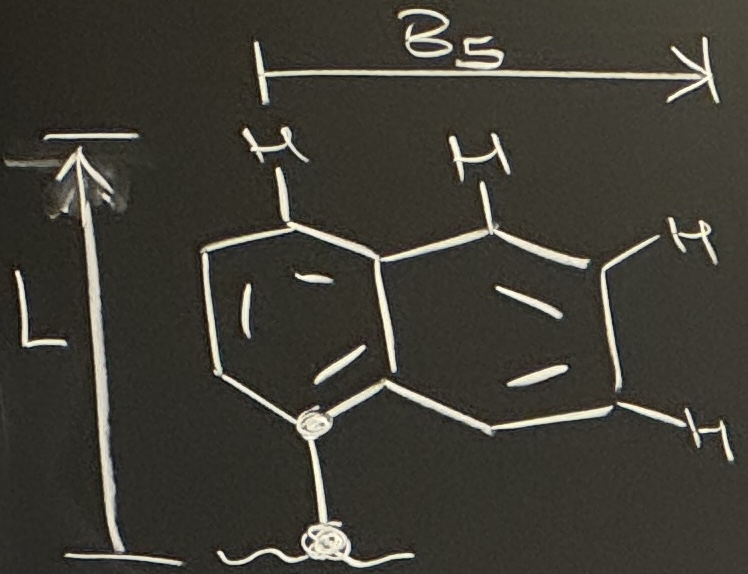
\includegraphics[width=0.8\linewidth]{sterimola.JPG}
            \caption{$L$/$B_5$ of 1-naphthyl.}
            \label{fig:sterimola}
        \end{subfigure}
        \begin{subfigure}[b]{0.23\linewidth}
            \centering
            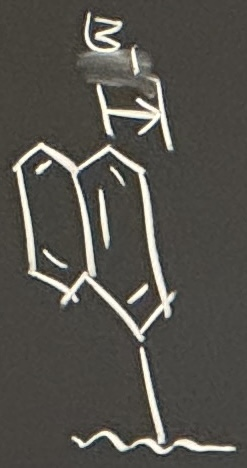
\includegraphics[width=0.4\linewidth]{sterimolb.JPG}
            \caption{$B_1$ of 1-naphthyl.}
            \label{fig:sterimolb}
        \end{subfigure}
        \begin{subfigure}[b]{0.23\linewidth}
            \centering
            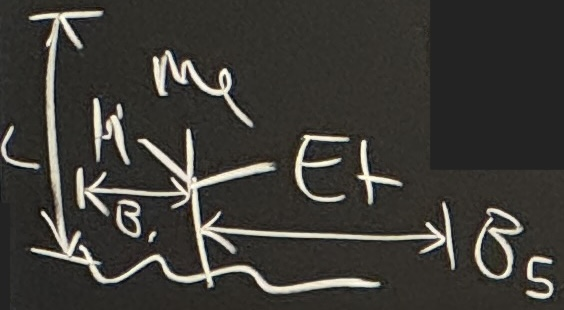
\includegraphics[width=0.8\linewidth]{sterimolc.JPG}
            \caption{$L$/$B_5$/$B_1$ of \emph{s}-butyl.}
            \label{fig:sterimolc}
        \end{subfigure}
        \caption{Sterimol parameters.}
        \label{fig:sterimol}
    \end{figure}
    \begin{itemize}
        \item These are our best steric parameters to date.
        \begin{itemize}
            \item They are very good at decoupling multiple dimensions of information.
            \item They can be calculated by a number of programs and websites.
        \end{itemize}
        \item Sterimol parameters narrow down what we mean by "size."
        \begin{itemize}
            \item For example, it's hard to say whether a tree or a car is bigger --- what do we mean by "big?" Trees have lots of empty space, cars are more dense, trees have more mass (in general), etc.
            \item The same is true of certain \ce{R} groups.
        \end{itemize}
        \item Sterimol parameters define the size of a substituent dimension by dimension.
        \begin{itemize}
            \item $L$ is the length (in \si{\angstrom}) from the "parent atom" to the end of the substituent, following the vector connecting the parent atom and the "start of the substituent" (Figure \ref{fig:sterimola}).
            \begin{itemize}
                \item The "parent atom" and "start of the substituent" are the circled atoms in Figure \ref{fig:sterimola}.
            \end{itemize}
            \item $B_5$ is the maximum size of the substituent along any vector perpendicular to $\vec{L}$ (Figure \ref{fig:sterimola}).
            % \begin{itemize}
            %     \item From your length vector, perpendicular to it, what is the maximum width in whatever direction would be the largest.
            % \end{itemize}
            \item $B_1$ is the minimum size of the substituent along any vector perpendicular to $\vec{L}$ (Figure \ref{fig:sterimolb}).
            \begin{itemize}
                \item Figure \ref{fig:sterimolb} is supposed to be a perspective drawing.
            \end{itemize}
        \end{itemize}
        \item Masha also draws the sterimol parameters on a \emph{sec}-butyl group (Figure \ref{fig:sterimolc}).
    \end{itemize}
    \item Some parameters account for both steric \emph{and} electronic effects.
    \begin{enumerate}
        \item \textbf{Taft parameters}.
        \item \textbf{Charton parameters}.
    \end{enumerate}
    \item \textbf{Taft parameter}: A measure of a substituent's ability to electronically activate or deactivate as well as sterically block or expose a reactive site. \emph{Given by}
    \begin{align*}
        \log(\frac{K_{\ce{X}}}{K_{\ce{H}}}) &= \rho^*\sigma^*+\delta E_s&
        \log(\frac{k_{\ce{X}}}{k_{\ce{H}}}) &= \rho^*\sigma^*+\delta E_s
    \end{align*}
    \begin{itemize}
        \item We can decouple the sterics and electronics by measuring $k$ or $K$ of both pathways.
        \begin{itemize}
            \item This is some good, honest physical organic chemistry that some people did.
        \end{itemize}
        \item $\rho^*\sigma^*$ is the \textbf{polar term}.
        \item $\delta E_s$ is the \textbf{steric term}
    \end{itemize}
    \item \textbf{Polar term}: The term governing electronics.
    \item \textbf{Steric term}: The term governing a substituent's ability to block $\pi^*$ because of its anomalous size.
    \begin{itemize}
        \item This definition is not necessarily universal; it's relevant to this reaction, specifically.
        \item In some reactions, the ability to block some other antibonding orbital will be more relevant.
    \end{itemize}
    \item Example: The hydrolysis of a methyl ester under basic and acidic conditions.
    \begin{figure}[H]
        \centering
        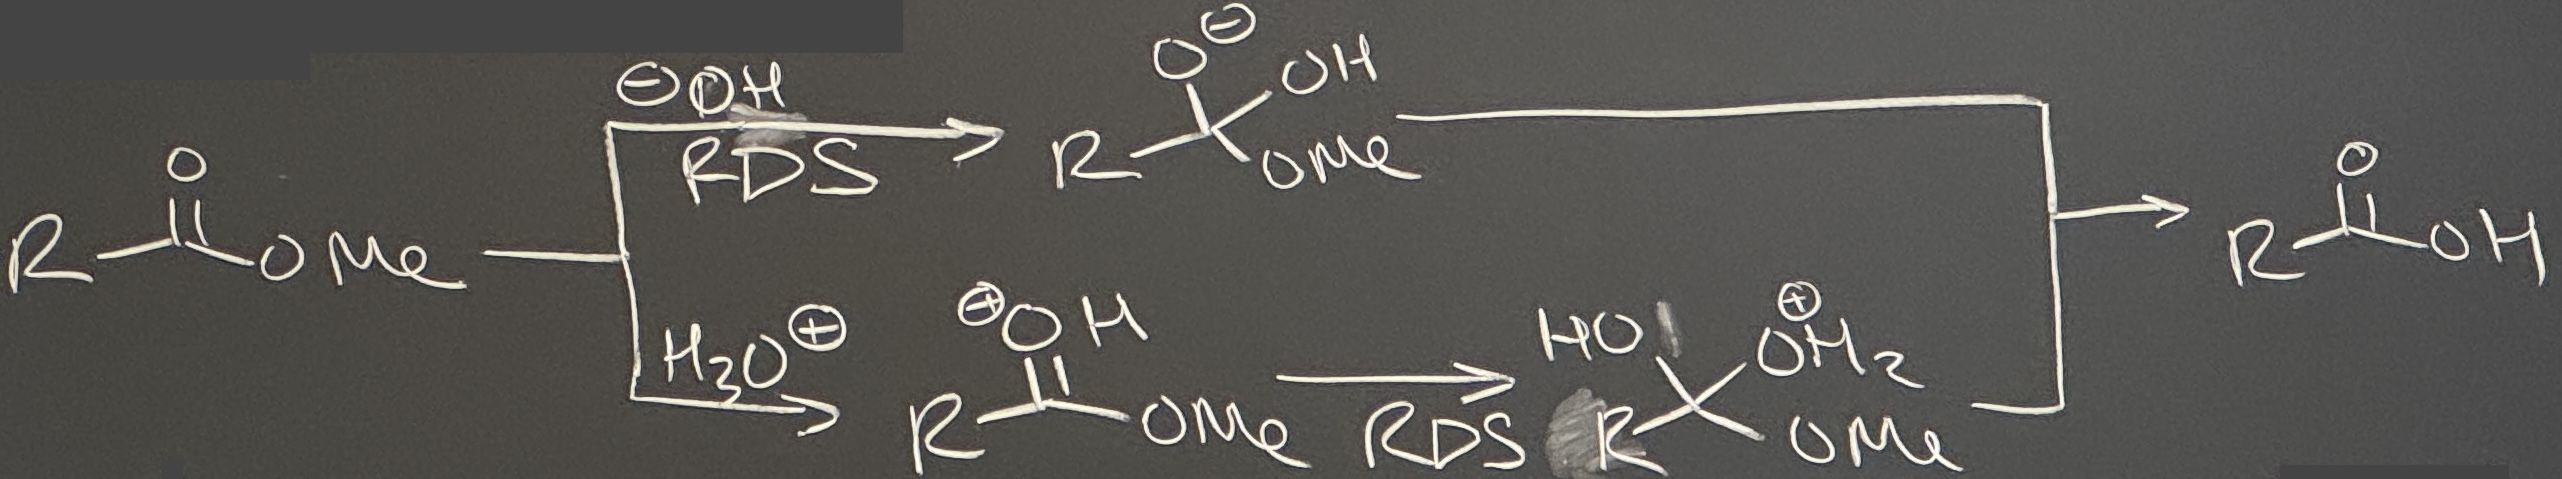
\includegraphics[width=0.7\linewidth]{taftPar.JPG}
        \caption{Taft parameters characterize ester hydrolysis.}
        \label{fig:taftPar}
    \end{figure}
    \begin{itemize}
        \item Under basic conditions, we have basically one step: Addition, then kicking out.
        \begin{itemize}
            \item The RDS is the hydroxide adding in.
            \item There is a negative charge buildup in the transition state.
            \item Therefore, the sterics of \ce{R} can block the addition and the electronics of \ce{R} might change the carbonyl's electrophilicity. In other words, both the sterics and electronics of \ce{R} matter.
        \end{itemize}
        \item Under acidic conditions, we could get protonation of the carbonyl followed by water addition to form the tetrahedral intermediate, and then elimination and deprotonation to the carboxylic acid product.
        \begin{itemize}
            \item The RDS is the water adding in.
            \item There is no charge buildup in the transition state (the charge is already included).
            \item Therefore, it's \emph{only} the sterics of \ce{R} that matter.
        \end{itemize}
    \end{itemize}
    \item \textbf{Charton parameter}: A refinement of $E_s$ with van der Waals radii. \emph{Also known as} \textbf{Charton modification of Taft parameters}.
    \item Taft and Charton are both a bit historical at this point, but we still need to know them in order to read the literature.
    \begin{itemize}
        \item Masha's never actually used them, but she does use sterimol.
    \end{itemize}
    \item We now move onto some steric parameters in catalysis; these were motivated by the need to quantify ligand size.
    \begin{figure}[h!]
        \centering
        \begin{subfigure}[b]{0.2\linewidth}
            \centering
            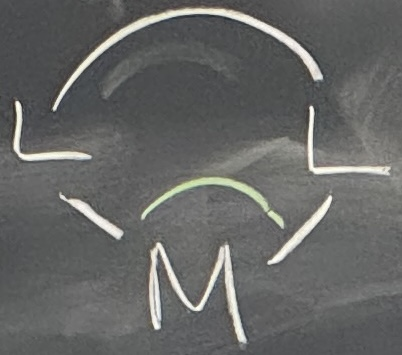
\includegraphics[width=0.4\linewidth]{stericPara.JPG}
            \caption{Bite angle.}
            \label{fig:stericPara}
        \end{subfigure}
        \begin{subfigure}[b]{0.2\linewidth}
            \centering
            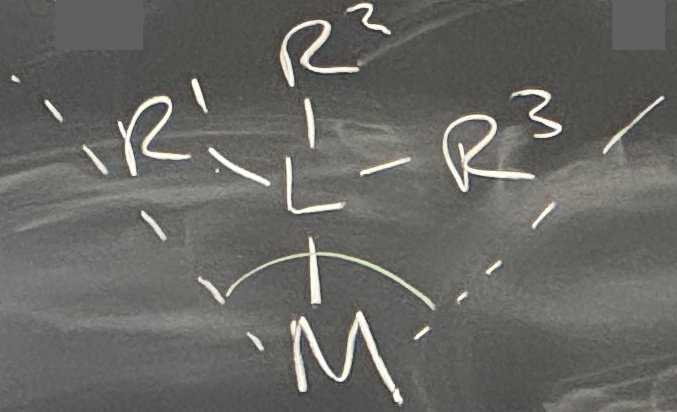
\includegraphics[width=0.85\linewidth]{stericParb.JPG}
            \caption{Cone angle.}
            \label{fig:stericParb}
        \end{subfigure}
        \begin{subfigure}[b]{0.2\linewidth}
            \centering
            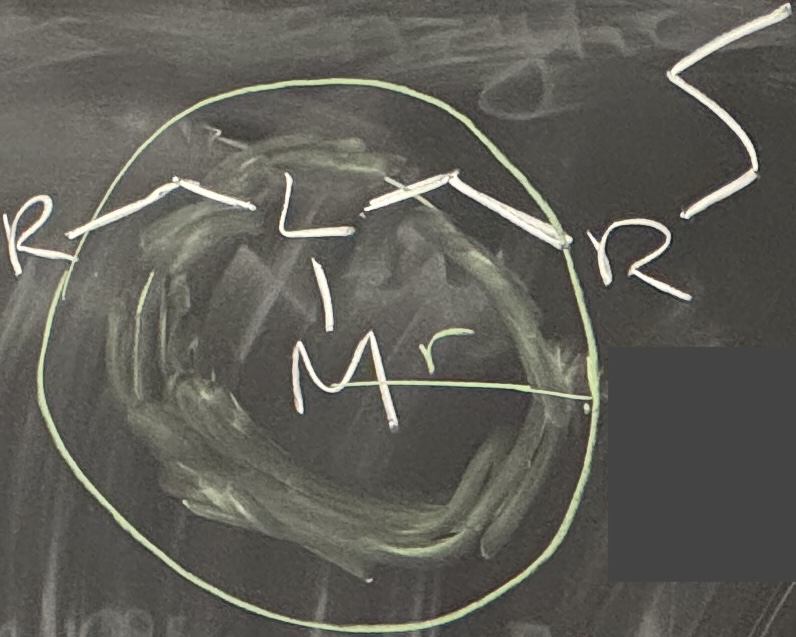
\includegraphics[width=0.95\linewidth]{stericParc.JPG}
            \caption{PBV.}
            \label{fig:stericParc}
        \end{subfigure}
        \caption{Steric parameters in catalysis.}
        \label{fig:stericPar}
    \end{figure}
    % \begin{enumerate}
    %     \item \textbf{Bite angle}.
    %     \item \textbf{Cone angle}.
    %     \item \textbf{Percent-buried volume}.
    % \end{enumerate}
    \item \textbf{Bite angle}: The \ce{L-M-L} angle for a bidentate ligand. \emph{Schematic} Figure \ref{fig:stericPara}.
    \begin{itemize}
        \item To reiterate: Bite angle is a metric of size for bidentate ligands \emph{only}.
        % \item You have a metal with L, L, and an abbreviated curved backbone. Then the bite angle is just the L-M-L angle!
        \item Naturally, bite angle depends significantly on the size of the metal.
        \begin{itemize}
            \item The example values below are all for the same metal.
            \item Historically, bite angles were reported for nickel.
        \end{itemize}
        \item Examples.
        \begin{itemize}
            \item DPPM, DPPE, and DPPP ligands have bite angles of \ang{73}, \ang{86}, and \ang{91}.
            \item TRANSphos has a \ang{180} angle so that it sits on either side of our catalys; really useful!
        \end{itemize}
        \item Bite angle correlates really well to a lot of reactivity, so it's good to know.
    \end{itemize}
    \pagebreak
    \item \textbf{Cone angle}: The angle from the metal to the outside \ce{R} groups, where \ce{L} is a monodentate ligand with three substituents. \emph{Schematic} Figure \ref{fig:stericParb}.
    \begin{itemize}
        \item To reiterate: Cone angle is a metric of size for monodentate ligands only.
        % \item If L has 3 substituents, this is the angle from the metal to the outside \ce{R} groups.
        \item Cone angle also (naturally) depends on the metal.
        \item Examples: Phosphane, trimethylphosphane, and triethylphosphane have \ang{87}, \ang{118}, and \ang{132}.
    \end{itemize}
    \item \textbf{Percent-buried volume}: The percent of the sphere around the metal occupied by the ligand, where the sphere has $r=\SI{3.5}{\angstrom}$ by default. \emph{Also known as} \textbf{PBV}. \emph{Schematic} Figure \ref{fig:stericParc}.
    \begin{itemize}
        \item The radius can be changed, though, because the ligand should fit mostly in the sphere.
        \item Examples: NHC ligands.
        \begin{itemize}
            \item If $\ce{R}=\ce{Me},\ce{{}^{\emph{i}}Pr},\ce{2,6{-}^{\emph{i}}PrPh}$, then $\text{PBV}=26,28,47$.
        \end{itemize}
        \item Example of when this is useful.
        \begin{itemize}
            \item If you want to block your metal, you need bigger \ce{R} groups.
            \item But if you just choose floppy alkyl chains, that might not really block the sphere because they'll just flop away.\footnote{Sometimes floppiness can be the point, though, as in my research with Santa!}
        \end{itemize}
        \item We should see these in papers.
        \item Use them in our work if we need!
    \end{itemize}
    \item This is it for regular parameters at this point.
    \item However, there's one more wrinkle: The case of multidimensional LFERs.
    \begin{figure}[h!]
        \centering
        \begin{subfigure}[b]{0.6\linewidth}
            \centering
            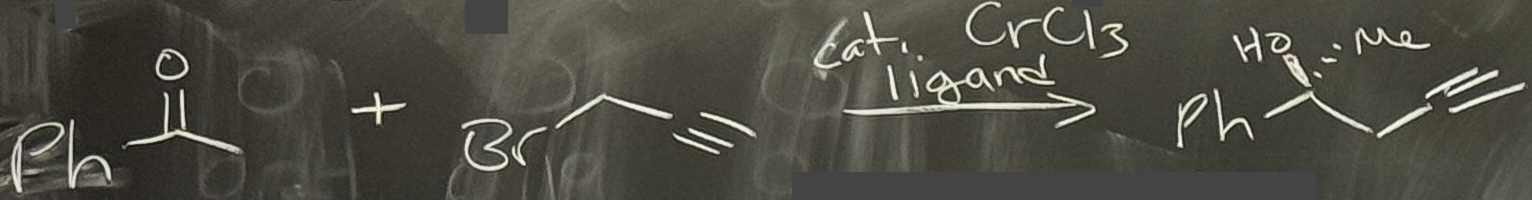
\includegraphics[width=0.9\linewidth]{multiLFERa.JPG}
            \caption{Reaction.}
            \label{fig:multiLFERa}
        \end{subfigure}
        \begin{subfigure}[b]{0.3\linewidth}
            \centering
            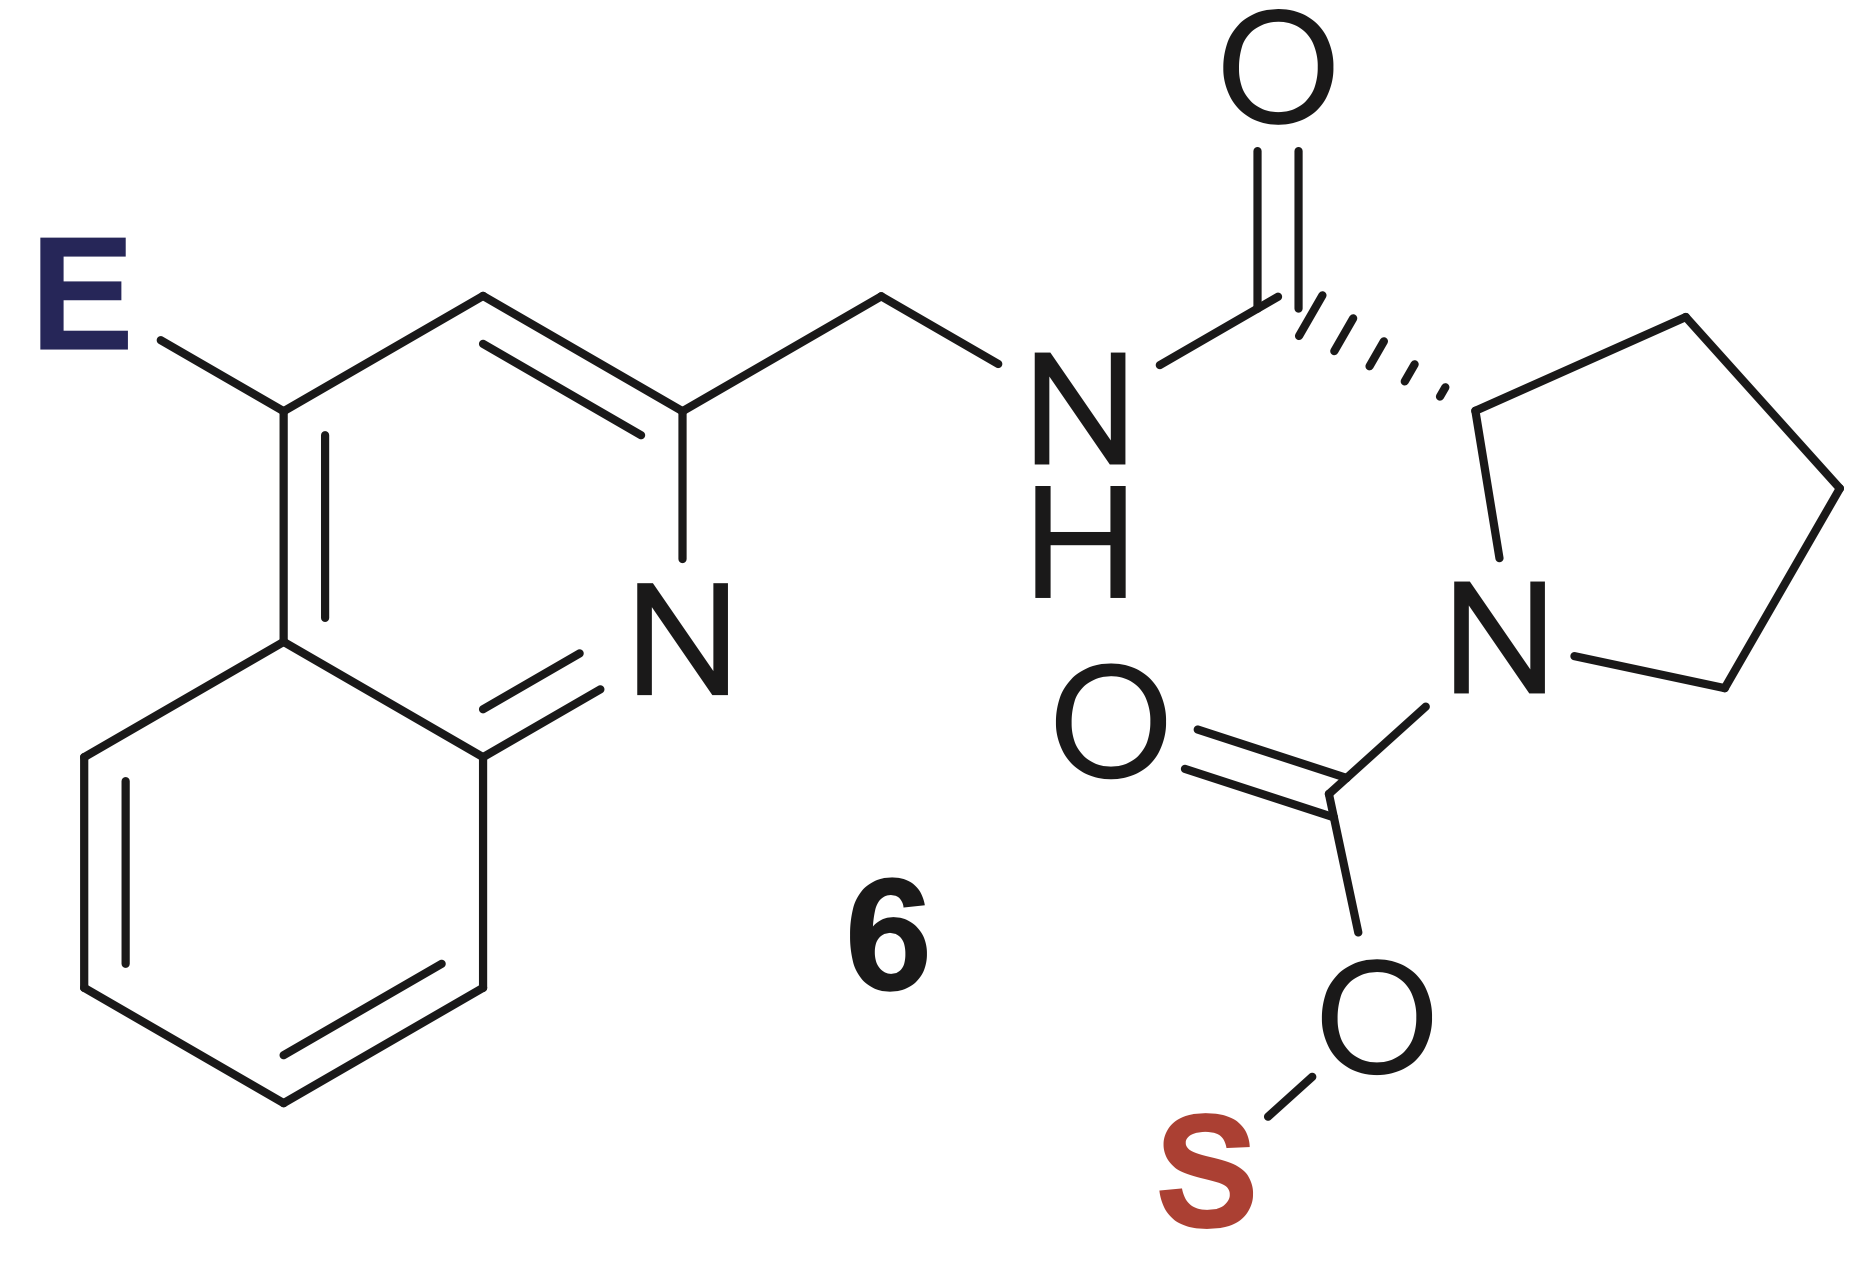
\includegraphics[width=0.7\linewidth]{multiLFERb.png}
            \caption{Ligand template.}
            \label{fig:multiLFERb}
        \end{subfigure}\\[2em]
        \begin{subfigure}[b]{0.58\linewidth}
            \centering
            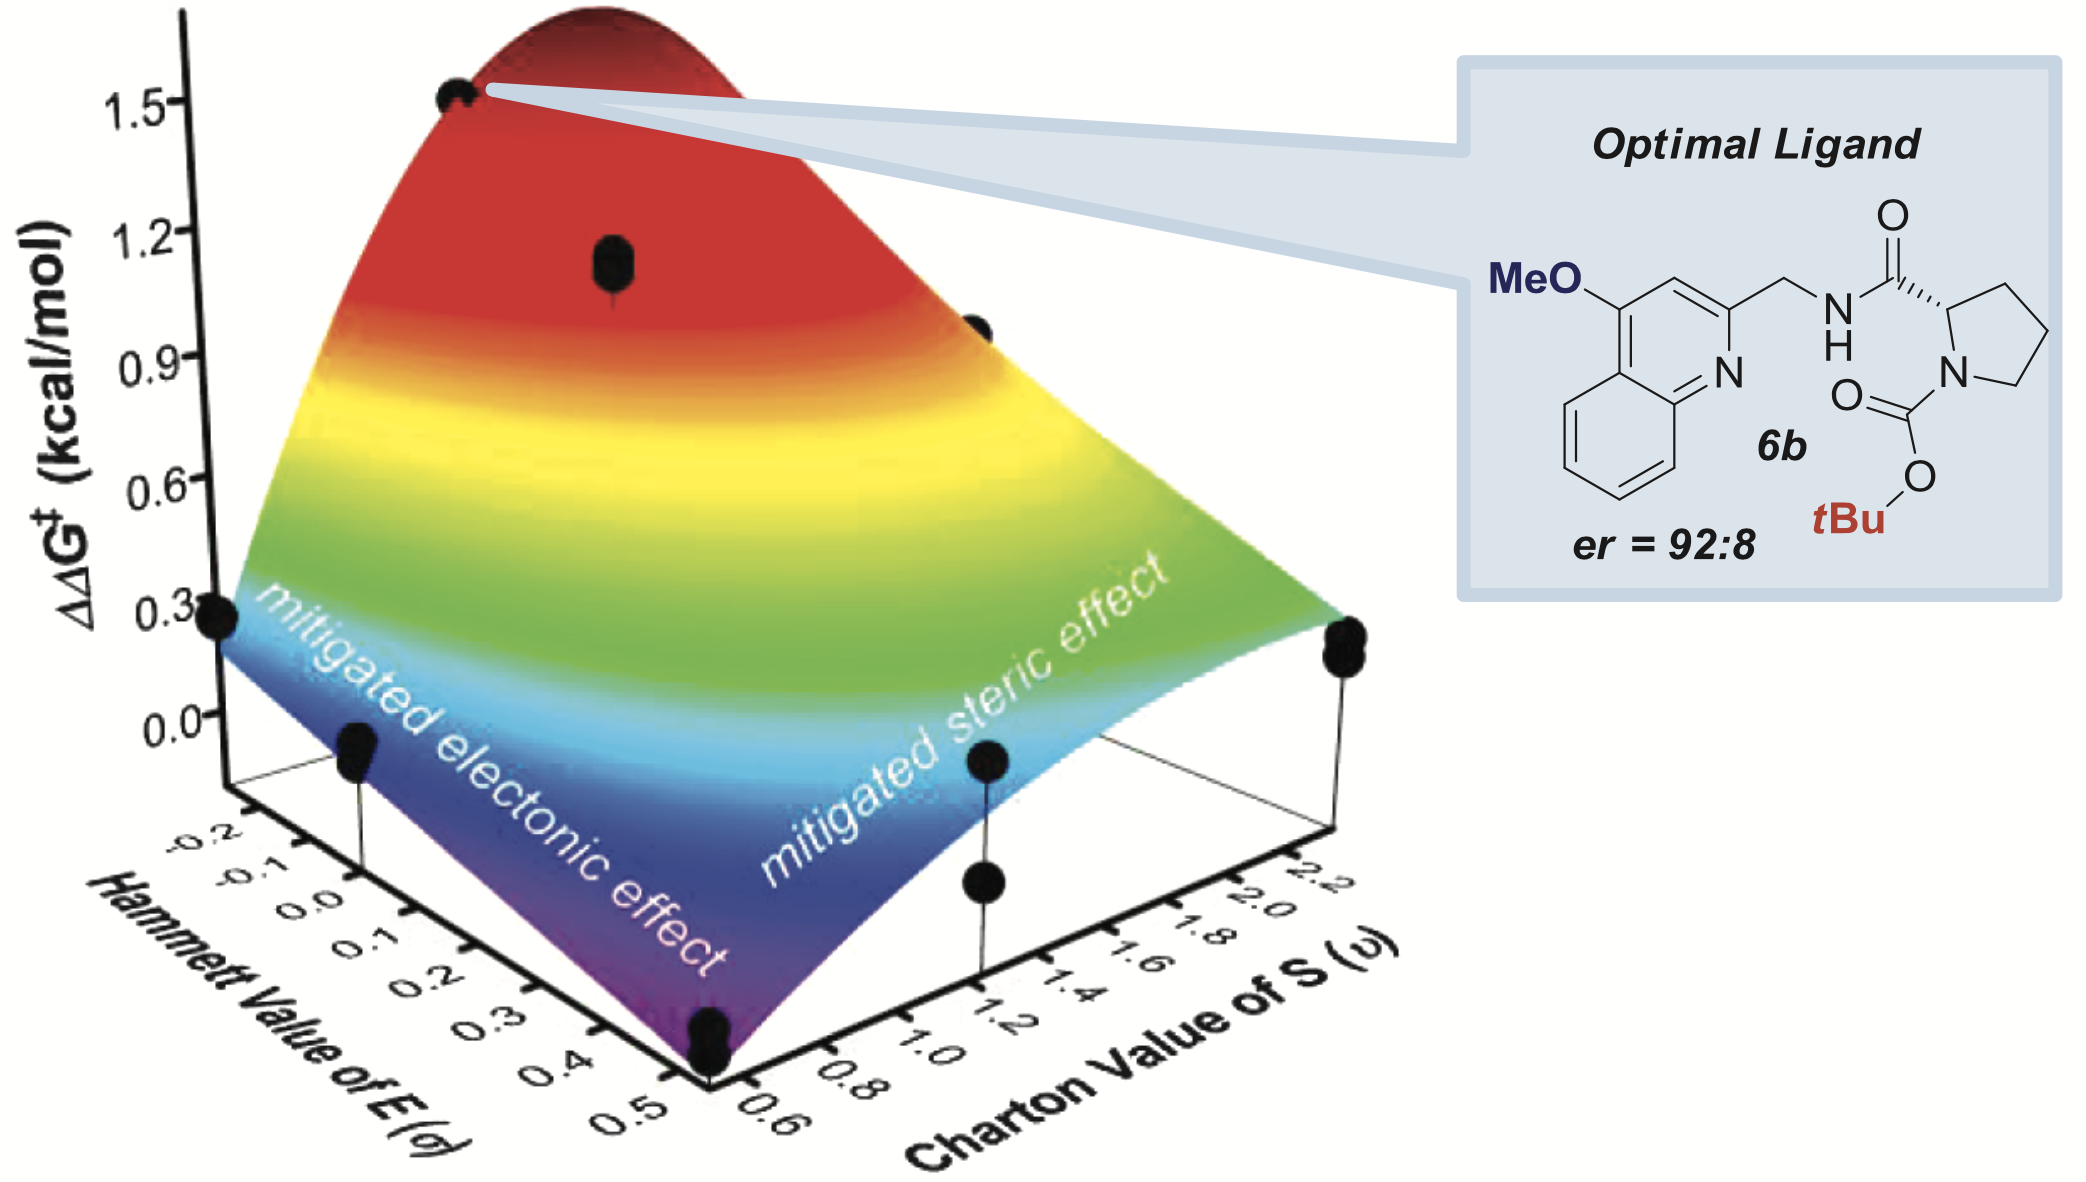
\includegraphics[width=0.9\linewidth]{multiLFERc.png}
            \caption{3D plot.}
            \label{fig:multiLFERc}
        \end{subfigure}
        \begin{subfigure}[b]{0.35\linewidth}
            \centering
            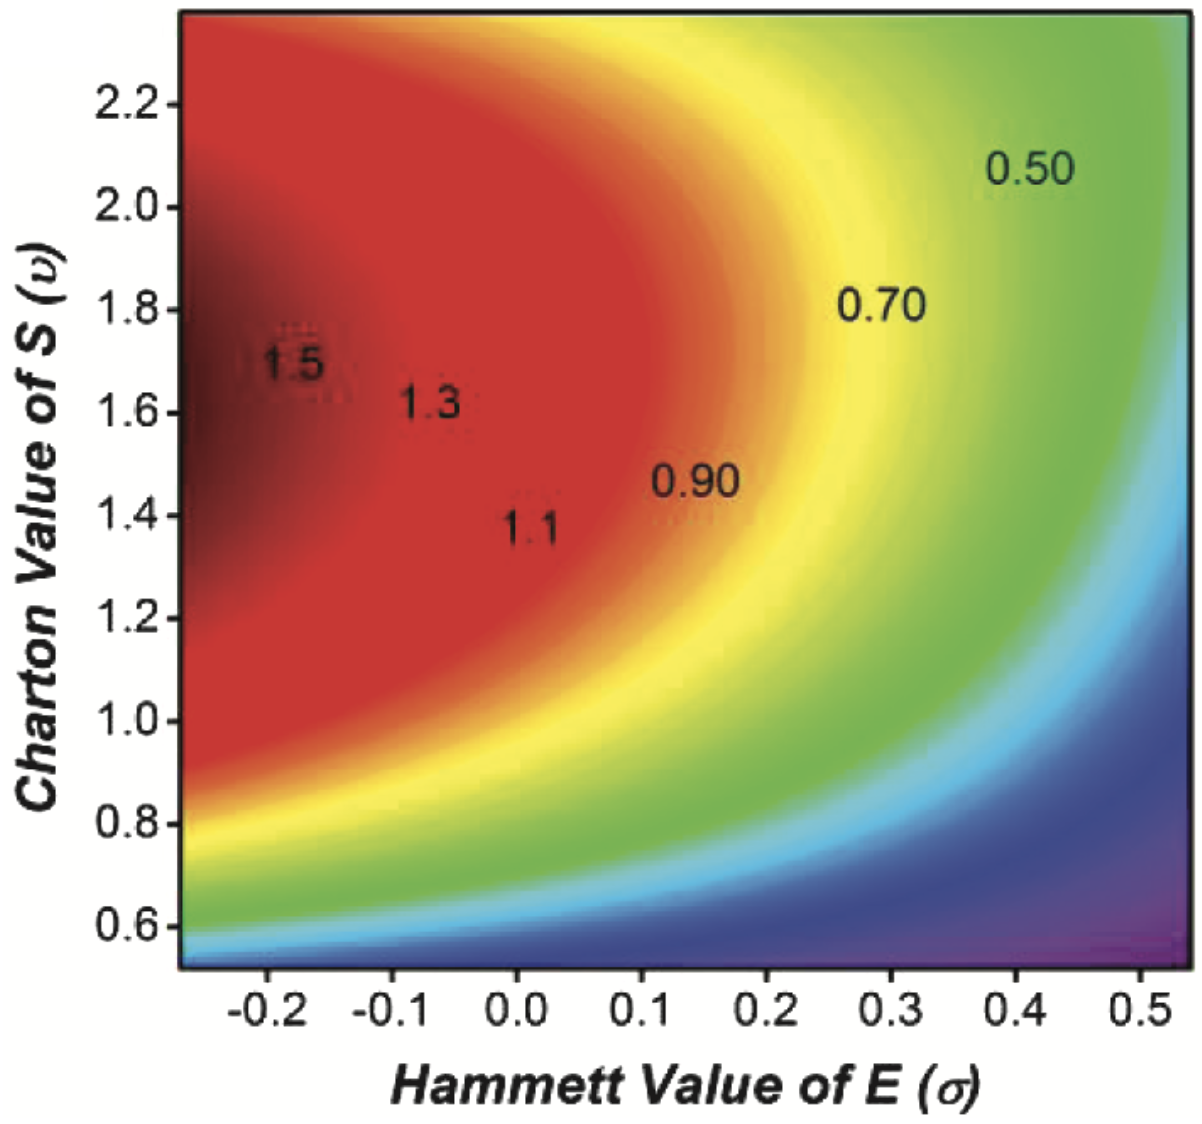
\includegraphics[width=0.9\linewidth]{multiLFERd.png}
            \caption{Contour map.}
            \label{fig:multiLFERd}
        \end{subfigure}
        \caption{Multidimensional LFERs.}
        \label{fig:multiLFER}
    \end{figure}
    \pagebreak
    \begin{itemize}
        \item To make sense of these, we use a higher-dimensional Hammett plot!
        \begin{itemize}
            \item Even this one step up gets us to multidimensional regression, which is the dawn of ML in chemistry.
            \item Back in the day, they called this multidimensional LFERs; today, we call it machine learning (ML).
        \end{itemize}
        \item Essentially, some substituents can have synergistic or interdependent effects.
        \begin{itemize}
            \item To conceptualize this kind of relationship, we model multiple parameters at once.
        \end{itemize}
        \item History.
        \begin{itemize}
            \item This work was pioneered by Matt Sigman at the University of Utah.
            \item Now a lot of other people have jumped in: Abby Doyle, Connor Coley, Masha, etc.
            \item "As this field gets bigger and bigger and hypier and hypier, no one should forget Matt. Don't come for Matt."
        \end{itemize}
        \item Example: Catalytic \ce{CrCl3} gets chelated to an asymmetric ligand (Figure \ref{fig:multiLFERb}), and then enantioselectively combines two things (Figure \ref{fig:multiLFERa}).
        \begin{itemize}
            \item Three variables to consider: Two independent variables, and one dependent variable.
            \begin{itemize}
                \item The authors varied the size of the substituent S, and measured its size with a Charton parameter, $\nu$.
                \item Simultaneously, they varied the electronics of the substituent E, and measured its EWG/EDG character with a Hammett parameter, $\sigma$.
                \item They measured the ee, from which they could calculate er, $\krel$, and finally $\Delta\Delta G^\ddagger$.
            \end{itemize}
            \item This all results in a 3D plot (Figure \ref{fig:multiLFERc}).
            \begin{itemize}
                \item The general shape is a sheet that's going up and down.
            \end{itemize}
            \item The contour map might be a bit easier to visualize (Figure \ref{fig:multiLFERd}).
            \begin{itemize}
                \item High ee toward the left and low ee toward the right.
            \end{itemize}
            \item We can also describe all this with an equation.
            \begin{equation*}
                \Delta\Delta G^\ddagger = -1.20+1.22E+2.84S-0.85S^2-3.79ES+1.25ES^2
            \end{equation*}
            \begin{itemize}
                \item The \textbf{cross terms} ($ES$ and $ES^2$) in this equation are particularly important; they are a mathematical demonstration of the interdependency between sterics and electronics.
                \item Thus, the $\Delta\Delta G^\ddagger$ depends on ligand sterics, electronics, and how those interact with each other.
                \item The original constant doesn't have chemical meaning, then electronic parameter, then two steric parameters, then two cross terms.
            \end{itemize}
            \item What's happening here in chemical terms is that electron-poor ligands are not very sensitive to sterics, but electron-rich ligands are.
            \begin{itemize}
                \item Note the difference in the curves in the back of the 3D plot and the front of the 3D plot. The back one (high EDG) is much more dependent on sterics! We want mid-sterics for highest ee.
                \item The front one isn't great.
            \end{itemize}
            \item So the best ligand is when \ce{E} is very electron-donating (\ce{OMe}) and S is big but not too big (\ce{{}^{\emph{t}}Bu}; not something huge like adamantyl).
            \item Reference: \textcite{bib:SigmanMulti}.
        \end{itemize}
    \end{itemize}
    \item Overall guide/overview to building your own multidimensional free energy relationship with more parameters: \textcite{bib:SigmanReview}.
    \begin{itemize}
        \item A very accessible read!
    \end{itemize}
\end{itemize}



\section{Office Hours (Jonathan)}
\begin{itemize}
    \item \marginnote{10/18:}What content will the exam cover?
    \begin{itemize}
        \item Everything through Hammett plots.
    \end{itemize}
    \item PSet 2, Q4?
    \begin{itemize}
        \item It is, indeed, a singlet carbene because the oxygen's $\pi$-donor ability travels through the $\pi$-network.
        \item The product only has \emph{two} stereocenters! The 3-membered ring is symmetric.
    \end{itemize}
\end{itemize}




\end{document}